\section{Problema inverso}\label{sec_prob_inv}

O problema inverso proposto neste trabalho é a estimativa da condutância térmica de contato $h_c$ na interface $\Gamma$ entre os corpos materiais
postos em contato $\Omega_1$ e $\Omega_2$, segundo o arranjo físico ilustrado na figura \ref{fig2}, conforme estabelecido na equação \eqref{eq:definicao_1}:
\begin{equation}
	h_c = \frac{q_c}{\Delta T_c}
\end{equation}

O fluxo de calor por unidade de área $q_c$ e o salto de temperatura $\Delta T_c$, ambos tomados na interface de contato, serão estimados de forma
indireta e não intrusiva, através do emprego do conceito de funcional de reciprocidade (FR), que será explicado na próxima seção.

A estimativa da CTC será feita através de medidas de temperaturas tomadas na superfície superior $\Gamma_0$ do corpo de prova, submetida a um fluxo
de calor por unidade de área $q$. As superfícies laterais $\Gamma_1$ e $\Gamma_2$ são mantidas termicamente isoladas, e a temperatura da superfície
inferior $\Gamma_\infty$ é mantida constante. As características geométricas e termofísicas dos corpos materiais em contato são conhecidas, a saber, as 
condutividades térmicas $k_1$ e $k_2$, bem como as dimensões $a$ e $b$ do corpo de prova e a curva $y = w(x)$, que descreve geometricamente a interface
de contato entre os corpos. 

\subsection{Definição do conceito de funcional de reciprocidade}

A ideia do funcional de reciprocidade teve origem a partir do trabalho de \cite{artigo_andrieux}, que introduziram o conceito de funcional de descontinuidade
de reciprocidade (do inglês, \textit{reciprocity gap functional}). Segundo os autores, a intenção era levantar informações sobre a estrutura interna de
um corpo a partir de grandezas medidas na fronteira deste corpo, posto que tais grandezas estivessem relacionadas a um fenômeno físico descrito por
equações diferenciais parciais elípticas. As informações obtidas, por sua vez, seriam caracterizações de descontinuidades, espaços vazios internos ou inclusões
de materiais, entendidas de forma geral como ``perturbações''. Os autores, no referido trabalho, concentraram-se no problema específico de identificação
de falhas planas no interior de corpos materiais.

Nesse sentido, a introdução de uma perturbação a um corpo material geraria uma resposta à aplicação de um campo escalar diferente da obtida se
essa perturbação não estivesse presente. Seja então um fluxo de uma grandeza escalar $\Phi_m$ imposto à fronteira externa $\partial\Omega$ de um corpo material
$\Omega$, e seja $U_m$ a medida de um campo escalar $u$ em equilíbrio, tomada na mesma fronteira (figura \ref{fig3}). Exemplos de grandezas dessa natureza são
temperatura e fluxo de calor, ou deformação e tensão. 
\begin{figure}[h!b]
\begin{center}
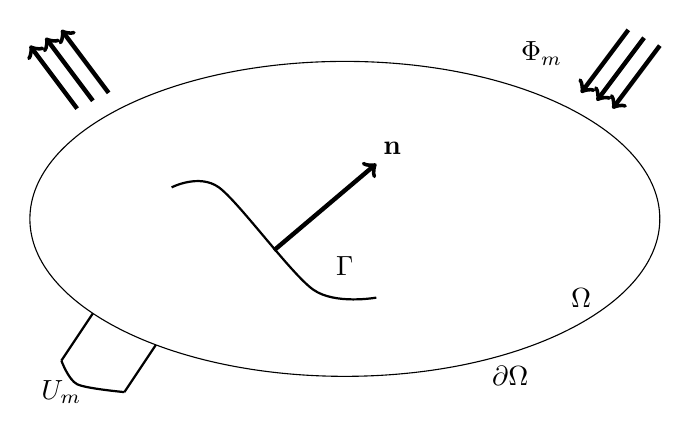
\begin{tikzpicture}[scale=1.0]
	\draw (0,0) ellipse (4cm and 2cm);
	\draw [->, ultra thick] (-3.4cm, 1.4cm) -- (-4.0cm, 2.2cm);
	\draw [->, ultra thick] (-3.2cm, 1.5cm) -- (-3.8cm, 2.3cm);
	\draw [->, ultra thick] (-3.0cm, 1.6cm) -- (-3.6cm, 2.4cm);
	\draw [->, ultra thick] (4.0cm, 2.2cm) -- (3.4cm, 1.4cm);
	\draw [->, ultra thick] (3.8cm, 2.3cm) -- (3.2cm, 1.5cm);
	\draw [->, ultra thick] (3.6cm, 2.4cm) -- (3.0cm, 1.6cm);
	\draw (2.5, 2.1) node {$\Phi_m$};
	\draw [thick] plot [smooth] coordinates {(-2.2, 0.4) (-1.6, 0.4) (-0.4, -0.9) (0.4, -1.0)};
	\draw (0.0, -0.6) node {$\Gamma$};
	\draw [->, ultra thick] (-0.9, -0.4) -- (0.4, 0.7);
	\draw (0.6, 0.9) node {$\mathbf{n}$};
	\draw (3.0, -1.0) node {$\Omega$};
	\draw (2.1, -2.0) node {$\partial\Omega$};
	\draw [thick] (-3.2cm, -1.2cm) -- (-3.6cm, -1.8cm);
	\draw [thick] (-2.4cm, -1.6cm) -- (-2.8cm, -2.2cm);
	\draw [thick] plot [smooth] coordinates {(-3.6cm, -1.8cm) (-3.4, -2.1) (-2.8cm, -2.2cm)};
	\draw (-3.6cm, -2.2cm) node {$U_m$};
\end{tikzpicture}
\caption{Corpo material $\Omega$ (adaptado de \citeauthor{artigo_andrieux}, \citeyear{artigo_andrieux})}
\label{fig3}
\end{center}
\end{figure}

A expressão que define o funcional de descontinuidade de reciprocidade, estabelecida por Andrieux e Ben Abda, é dada por:
\begin{align}
	RG(v) = \int_{\partial\Omega} \left( \Phi_m v - U_m \nabla v \cdot \mathbf{n} \right) \label{definicao_rgap}
\end{align}
onde $v$ é um outro campo potencial em equilíbrio em $\Omega$.

Os autores afirmam que quando não há descontinuidades no interior de $\Omega$, a integral \eqref{definicao_rgap} se anula. Desse modo, o funcional de descontinuidade de reciprocidade
forneceria uma medida do desvio provocado num campo escalar $u$ no corpo $\Omega$ submetido a um fluxo $\Phi_m$ em sua superfície, se esse corpo
possuir uma descontinuidade $\Gamma$ em seu interior.

É importante destacar que a integral \eqref{definicao_rgap} é calculada sobre o contorno da fronteira do corpo material $\Omega$, onde as grandezas envolvidas devem
ser efetivamente conhecidas. Assim, é possível inferir características no interior do corpo a partir de medições tomadas em seu contorno.

\subsection{Aplicação do funcional de reciprocidade na dedução da expressão da estimativa da condutância térmica de contato}\label{secao_sobre_fr}

Baseados no conceito de funcional de descontinuidade de reciprocidade, \cite{reciproc_2} apresentaram um trabalho pioneiro em que estabeleceram uma
técnica não intrusiva e não iterativa para solução de problemas inversos de transferência de calor, voltada para a estimativa da condutância térmica de
contato (CTC) entre dois corpos. A metodologia aplicada nesta dissertação, baseada no referido trabalho e em trabalhos posteriores em que aquele conceito
foi utilizado \citep{artigo_padilha_3}, será descrita nos parágrafos a seguir. 

\cite{reciproc_2} adaptaram o termo original definido em \eqref{definicao_rgap} para o problema formulado na seção \ref{sec_formulacao_direta},
introduzindo o conceito de funcional de reciprocidade (FR) através da seguinte expressão:
\begin{align}
	\Re(F) = \int_{\Gamma_0}\left[\left(\frac{-q}{k_1}\right)F - Y\frac{\partial F}{\partial\mathbf{n_1}}\right]d\Gamma_0
	\label{def_funcional_reciprocidade}
\end{align}
onde $F$ é uma função associada a um campo potencial auxiliar em equilíbrio em $\Omega_1$, $k_1$ é a condutividade térmica do material $\Omega_1$, $q$ é o fluxo de calor por unidade de área
aplicado na superfície externa $\Gamma_0$ e $Y$ são medidas de temperatura tomadas na mesma superfície $\Gamma_0$. O vetor $\mathbf{n_1}$ é o vetor normal à superfície
$\Gamma_0$ e apontando para fora do contorno do material $\Omega_1$.

De forma análoga à equação \eqref{definicao_rgap}, a equação \eqref{def_funcional_reciprocidade} permite medir a alteração do campo de temperatura
gerado por um fluxo de calor por unidade de área $q$ aplicado na superfície externa $\Gamma_0$ do material compósito $\Omega$ devido à existência
de uma descontinuidade $\Gamma$ em seu interior; essa alteração está relacionada à existência de uma resistência térmica de contato nessa interface. No caso de não haver descontinuidade
em $\Omega$, a integral \eqref{def_funcional_reciprocidade} se anula.

Em seu trabalho, \cite{reciproc_2} formulam dois problemas difusivos para determinação de duas classes de funções auxiliares $F_1$ e $G_1$, no mesmo domínio físico da região compreendida
por $\Omega_1$. Os problemas formulados são análogos ao problema de difusão de temperatura formulado em \eqref{harm_T1}--\eqref{cc_T1_5}, porém empregando condições de contorno apropriadas, que
serão detalhadas na seção \ref{secao_probs_aux}.

Através dessas condições de contorno, os autores demonstram as seguintes identidades:
\begin{align}
	k_1 \int_{\Gamma_0}\left[\left(\frac{-q}{k_1}\right)F_1 - Y\frac{\partial F_1}{\partial\mathbf{n_1}}\right]d\Gamma_0
	=
	\int_\Gamma k_1 \frac{\partial F_1}{\partial\mathbf{n_1}}\left(T_1 - T_2\right)d\Gamma
	\label{identidade_T}
\end{align}
\begin{align}
	k_1 \int_{\Gamma_0}\left[\left(\frac{-q}{k_1}\right)G_1 - Y\frac{\partial G_1}{\partial\mathbf{n_1}}\right]d\Gamma_0
	=
	\int_\Gamma -k_1 G_1 \frac{\partial T_1}{\partial\mathbf{n_1}}d\Gamma
	\label{identidade_q}
\end{align}

Os termos à esquerda das equações \eqref{identidade_T} e \eqref{identidade_q} são, a menos da constante multiplicativa $k_1$, a definição do funcional de reciprocidade para as 
funções auxiliares $F_1$ e $G_1$.

As integrais à direita têm um significado importante. É possível observar que elas são calculadas \textit{ao longo da interface de contato} $\Gamma$. O termo
$T_1 - T_2$ é exatamente \textit{o salto de temperatura através da interface} $\Gamma$, enquanto que o termo $\displaystyle-k_1 \frac{\partial T_1}{\partial\mathbf{n_1}}$
é exatamente \textit{o fluxo de calor por unidade de área através da interface} $\Gamma$ (cf. equação \eqref{eq:definicao_2}). Desse modo, as identidades \eqref{identidade_T} e \eqref{identidade_q}
relacionam \textit{as medidas
do salto de temperatura e de fluxo de calor na interface} $\Gamma$ -- grandezas cuja razão fornece a RTC sobre a interface -- com \textit{as medidas de temperatura} $Y$ \textit{tomadas na superfície} $\Gamma_0$.

Estas mesmas integrais também podem ser interpretadas à luz dos conceitos de Álgebra Linear \citep{livro_axler}. Sob esse ponto de vista, os termos
$\displaystyle k_1 \frac{\partial F}{\partial\mathbf{n_1}}$, $T_1 - T_2$, $G$ e $\displaystyle-k_1 \frac{\partial T_1}{\partial\mathbf{n_1}}$ podem ser identificados como funções pertencentes a um espaço
linear de funções, denotado por $L^2(\Gamma)$, em que se define a operação de produto interno como segue:
\begin{align}
	\langle f_1, f_2\rangle_{L^2(\Gamma)} = \int_\Gamma f_1(\Gamma) f_2(\Gamma) d\Gamma \label{definicao_innner_product}
\end{align} 
onde $f_1$ e $f_2$ são funções reais, contínuas por partes, definidas ao longo do contorno $\Gamma$ sobre o qual é calculada a integral. A norma de uma
função, que é uma métrica análoga ao ``comprimento'' ou ``distância'', é definida nesse espaço linear como\footnote{A partir desse ponto, o subscrito ${L^2(\Gamma)}$ será
subentendido nas transcrições de produtos internos, para fins de simplificação gráfica das equações.}:
\begin{align}
	\norm{f} = \sqrt{\langle f, f\rangle}
\end{align}

A partir de parametrizações convenientes dos problemas difusivos auxiliares, é possível levantar duas famílias de funções auxiliares $F_{1,j}, j=1,2,\ldots N_1$
e $G_{1,j}, j=1,2,\ldots N_2$. Assim, através da definição de produto interno em \eqref{definicao_innner_product} e da definição de funcional de reciprocidade em \eqref{def_funcional_reciprocidade},
as identidades \eqref{identidade_T} e \eqref{identidade_q} podem ser reescritas como:
\begin{align}
	k_1 \Re(F_{1,j})
	=
	\left\langle \left[T_1 - T_2\right]_\Gamma, \beta_j\right\rangle
	\label{identidade_T_inner}
\end{align}
\begin{align}
	k_1 \Re(G_{1,j})
	=
	\left\langle  -k_1 \frac{\partial T_1}{\partial\mathbf{n_1}}\bigg|_\Gamma, \gamma_j\right\rangle
	\label{identidade_q_inner}
\end{align}
onde
\begin{align}
	\beta_j = k_1 \frac{\partial F_{1,j}}{\partial\mathbf{n_1}}\bigg|_\Gamma \label{expressao_define_beta}
\end{align}
\begin{align}
	\gamma_j = G_{1,j}\big|_\Gamma \label{expressao_define_gamma}
\end{align}

Com base no trabalho de \cite{artigo_padilha_3}, será proposto um procedimento de parametrização de condições de contorno dos problemas auxiliares de modo que as funções
$\beta_j, j=1,2,\ldots N_1$ e $\gamma_j, j=1,2,\ldots N_2$ formem dois conjuntos ortonormais, isto é:
\begin{align}
	\left\langle  \beta_m, \beta_n \right\rangle = \left\lbrace
		\begin{matrix}
		0, & m \neq n \\
		1, & m = n 
		\end{matrix}
	\right.
\end{align}
\begin{align}
	\left\langle  \gamma_m, \gamma_n \right\rangle = \left\lbrace
		\begin{matrix}
		0, & m \neq n \\
		1, & m = n 
		\end{matrix}
	\right.
\end{align}

Nessas condições, cada um dos conjuntos define um subespaço linear contido no espaço linear $L^2(\Gamma)$. Os subespaços lineares gerados pela bases
ortonormais $\beta_j$ e $\gamma_j$ serão denotados respectivamente por $L^2(\Gamma, \beta)$ e $L^2(\Gamma, \gamma)$.

Por definição, a \textit{projeção ortogonal} de uma função $f$ pertencente ao espaço linear $L^2(\Gamma)$ sobre o subespaço linear $L^2(\Gamma, \epsilon)$
gerado por uma base ortonormal $\epsilon_j, j=1,2,\ldots,N$ é dada por:
\begin{align}
	P_{L^2(\Gamma, \epsilon)}[f] = \sum_{j=1}^N \left\langle f, \epsilon_j \right\rangle \epsilon_j
\end{align}

A projeção ortogonal provê uma forma aproximada de se representar uma função $f$ como combinação linear dos elementos de uma base ortonormal de
funções. Com efeito, seja $g$ uma função em $L^2(\Gamma, \epsilon)$, e que portanto pode ser expandida como uma combinação linear dos elementos da base $\epsilon_j$. Uma métrica de
avaliação da ``distância'' entre as funções $f$ e $g$ é dada pela norma da diferença entre essas funções. O menor valor possível para essa norma ocorre
quando a função $g$ for a projeção ortogonal de $f$ sobre $L^2(\Gamma, \epsilon)$ \citep{livro_axler}. Ou seja,
\begin{align}
	\norm{f - P_{L^2(\Gamma, \epsilon)}[f]} \le \norm{f - g}, \forall g \in L^2(\Gamma, \epsilon)
\end{align}

Dessa forma, o salto de temperatura e o fluxo de calor por unidade de área na interface $\Gamma$ podem ser representados de forma aproximada através de projeções
ortogonais sobre os subespaços lineares $L^2(\Gamma, \beta)$ e $L^2(\Gamma, \gamma)$ respectivamente:
\begin{align}
[T_1 - T_2]_\Gamma \approx \sum_{j=1}^{N_1} \left\langle  \left[T_1 - T_2\right]_\Gamma, \beta_j \right\rangle \beta_j
\end{align}
\begin{align}
	- k_1 \frac{\partial T_1}{\partial\mathbf{n_1}}\bigg|_\Gamma \approx \sum_{j=1}^{N_2} \left\langle  -k_1 \frac{\partial T_1}{\partial\mathbf{n_1}}\bigg|_\Gamma, \gamma_j \right\rangle \gamma_j
\end{align}

Aplicando as identidades \eqref{identidade_T_inner} e \eqref{identidade_q_inner} às equações acima, e assumindo que as projeções ortogonais representam
de forma razoável as funções correspondentes, pode-se escrever:
\begin{align}
	[T_1 - T_2]_\Gamma = \sum_{j=1}^{N_1} k_1 \Re(F_{1,j}) \beta_j \label{resultado_1}
\end{align}
\begin{align}
	- k_1 \frac{\partial T_1}{\partial\mathbf{n_1}}\bigg|_\Gamma = \sum_{j=1}^{N_2} k_1 \Re(G_{1,j}) \gamma_j \label{resultado_2}
\end{align}

Finalmente, substituindo os resultados obtidos em \eqref{resultado_1} e \eqref{resultado_2} na definição de condutância térmica de contato,
\eqref{eq:definicao_3}, obtemos a seguinte relação:
\begin{align}
	& h_c % = \frac{- k_1 \displaystyle\frac{\partial T_1}{\partial\mathbf{n_1}}\bigg|_\Gamma}{[T_1 - T_2]_\Gamma} 
	= \frac{\displaystyle\sum_{j=1}^{N_2} \Re(G_{1,j}) \gamma_j}{\displaystyle\sum_{j=1}^{N_1} \Re(F_{1,j}) \beta_j}
	\label{equacao_definicao_f_r}
\end{align}
%ou, de forma mais explícita:
%\begin{align}
%	& h_c % = \frac{- k_1 \displaystyle\frac{\partial T_1}{\partial\mathbf{n_1}}\bigg|_\Gamma}{[T_1 - T_2]_\Gamma} 
%	= \frac{\displaystyle\sum_{j=1}^{N_2} \gamma_j\int_{\Gamma_0}\left[\left(\frac{-q}{k_1}\right)G_{1,j} - Y\frac{\partial G_{1,j}}{\partial\mathbf{n_1}}\right]d\Gamma_0}{\displaystyle\sum_{j=1}^{N_1} \beta_j \int_{\Gamma_0}\left[\left(\frac{-q}{k_1}\right)F_{1,j} - Y\frac{\partial F_{1,j}}{\partial\mathbf{n_1}}\right]d\Gamma_0}
%	\label{equacao_definicao_f_r_expl}
%\end{align}

A expressão \eqref{equacao_definicao_f_r} permite calcular a estimativa da distribuição da CTC ao longo da interface de contato $\Gamma$, conhecendo-se
a distribuição de temperaturas $Y$ medidas na face externa superior do arranjo físico da figura \ref{fig2}, eliminando assim a necessidade prévia de
se conhecer informações e características internas do corpo de prova, tais como rugosidade entre as superfícies em contato, pressão de contato, ou
o fluido presente no interstício. As determinações do salto de temperatura e fluxo de calor por unidade de área na interface de contato são feitas de forma indireta, através
das expansões em funções ortonormais expressas em \eqref{resultado_1} e \eqref{resultado_2}, o que indica o caráter não intrusivo da técnica.

Quanto ao aspecto numérico-computacional, é possível notar que as integrais que fornecem os funcionais de reciprocidade só precisam ser calculadas
uma única vez, para uma determinada caracterização geométrica e termofísica do problema. As classes de funções $F_{1,j}$ e $G_{1,j}$, obtidas através da resolução dos
problemas difusivos auxiliares, dependem unicamente das
características geométricas (comprimento e largura do corpo de prova, e a curva $y = w(x)$ que descreve o formato da interface)
e termofísicas (condutâncias térmicas $k_1$ e $k_2$ dos materiais em contato). Por essa razão, o método é classificado como não iterativo, visto que
a obtenção da estimativa da CTC em algum ponto sobre a interface se resume à substituição dos valores de $\beta_j$ e $\gamma_j$ avaliados naquele
ponto nos somatórios da equação \eqref{equacao_definicao_f_r}.

Por último, é importante destacar que a expressão \eqref{equacao_definicao_f_r} permite a estimativa da CTC para qualquer formato de interface $\Gamma$,
desde que se conheça a sua descrição analítica representada pela curva $y = w(x)$. O caso particular em que a interface é plana e paralela às bases do corpo
de prova foi resolvido analiticamente por \cite{tese_padilha}.

% \subsection{Comentários sobre o caso particular de interface de contato plana}
% 
% O problema inverso definido pelo arranjo físico representado na figura \ref{fig2}, juntamente com as equações \eqref{harm_T1} -- \eqref{cc_T1_5}, é uma
% generalização de um problema mais simples em que a interface de contato é um plano paralelo às faces inferior e superior do corpo de prova, conforme
% ilustrado na \ref{fig4}.
